\subsection{Cross-Database Experiments}
I firstly pre-trained my models on the Finger Knuckle V1 Database, and then fine-tuned models on the Finger Knuckle V3 Database (with deformable). I use these kind training method, and use these models to test performance on the Index Finger Knuckle of Hand Dorsal Image and Tsinghua Finger Knuckle Database as a cross database experiment. The label in the finger curve, the content in parentheses indicates the training samples. Such as RFN-WS(1-104), it uses 1-104 subjects of Finger Knuckle V3 Database to train models. Updated ROC Curve and CMC Curve with RFNet, EfficientNet and DeConvRFNet. \textcolor{red}{For the ROC curve, I add EfficientNetV2-S model performance.}

\subsubsection{Index Finger Knuckle of Hand Dorsal Image}

\begin{figure}[H]
	\centering
	\begin{subfigure}[b]{0.8\linewidth}
		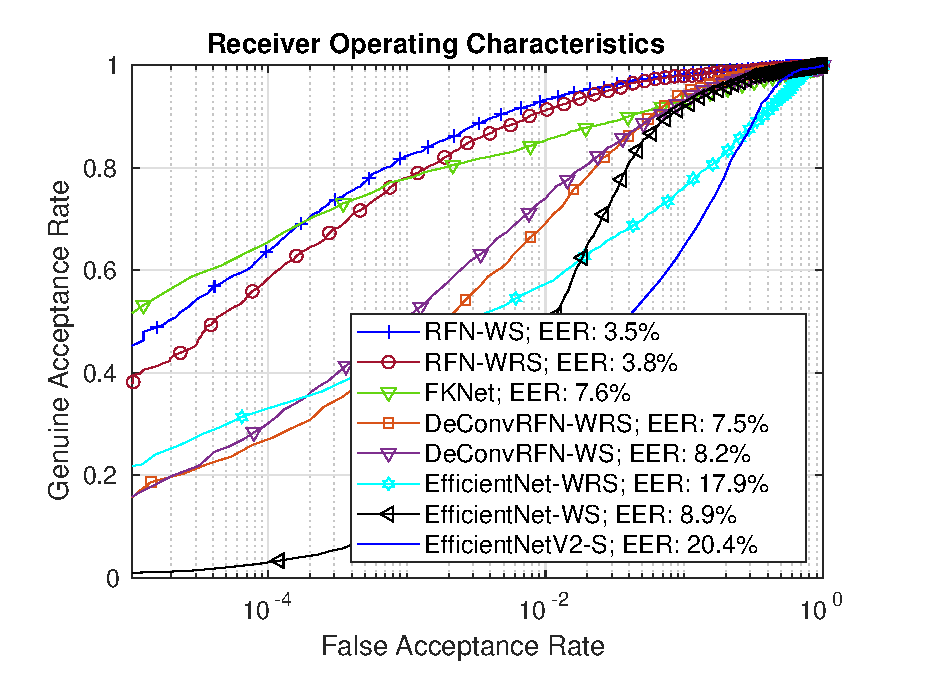
\includegraphics[width=\linewidth]{Figures/add-efficientv2-s/cross-hd-roc_compare_new.eps}
	\end{subfigure}
    \begin{subfigure}[b]{0.8\linewidth}
		\includegraphics[width=\linewidth]{Figures/fknet/cross-hd-cmc.eps}
	\end{subfigure}
\end{figure}

The database totally has 712 subjects, and each subject has 5 samples. Therefore, it will have $712*5$ genuine matching scores and $712*711*5$ imposter matching scores. From the cure, the performance of RFN-WS and RFN-WRS is similar, and the RFN-WS is slightly better than RFN-WRS while using the same training samples. Updated ROC Curve and CMC Curve with RFNet, EfficientNet and DeConvRFNet.\textcolor{red}{For the ROC curve, I add EfficientNetV2-S model performance.}


\subsubsection{Tsinghua Finger Knuckle Database}
\begin{figure}[H]
	\centering
	\begin{subfigure}[b]{0.8\linewidth}
		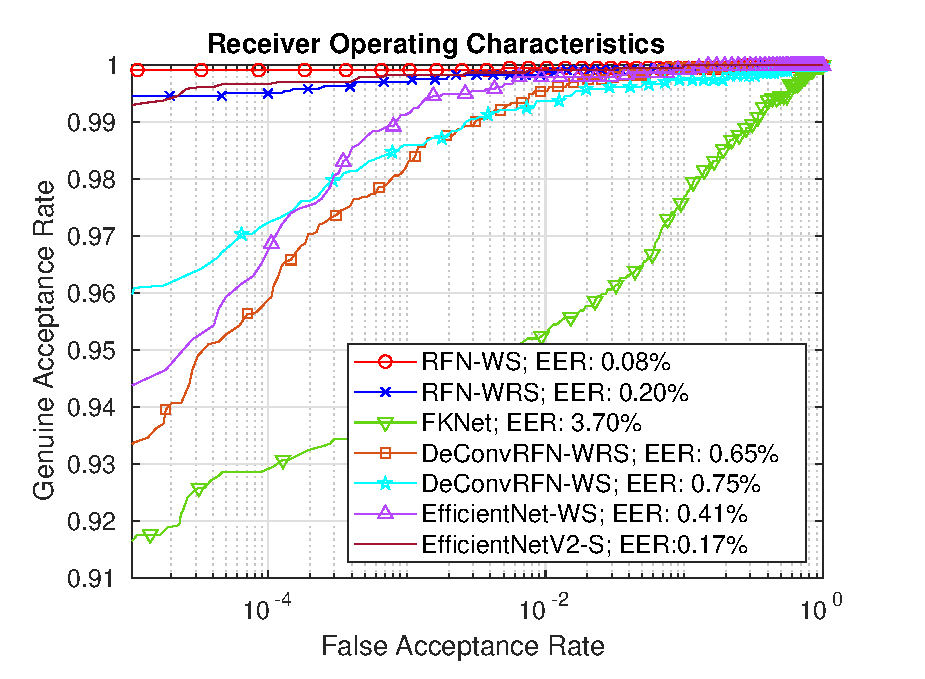
\includegraphics[width=\linewidth]{Figures/add-efficientv2-s/cross-thu-roc_compare_new.eps}
	\end{subfigure}
    \begin{subfigure}[b]{0.8\linewidth}
		\includegraphics[width=\linewidth]{Figures/fknet/cross-thu-cmc.eps}
	\end{subfigure}
\end{figure}

The database has 610 subjects, and each subject can offer 4 samples. Then as the cross database experiment, it will have $610*4$ genuine matching scores and $610*609*4$ imposter matching scores. In this database, all models can get very high matching performance from the table and figure.

\subsection{Challenging Protocol Experiments}
I have a challenging protocol experiment on the 2d image of 3d finger knuckle database. The experiment protocol is similar with the "Experiments Results using Challenging Protocol".

\subsubsection{One-session}
I pre-trained my model on Finger Knuckle V1 Database. As for the one-session experiment, I was firstly fine-tuning my model on the second session forefinger dataset which has 190 subjects, and then use the all-to-all protocol to evaluate matching accuracy on the first session of forefinger and middle finger, then combine both of them.

\begin{figure}[H]
    \centering
    \begin{subfigure}[b]{0.4\linewidth}
        \includegraphics[width=\linewidth]{Figures/challenging/one-session-forefinger.png}
        \caption{Index Finger}
    \end{subfigure}
    \begin{subfigure}[b]{0.4\linewidth}
        \includegraphics[width=\linewidth]{Figures/challenging/one-session-middle.png}
        \caption{Middle Finger}
    \end{subfigure}
    \begin{subfigure}[b]{0.4\linewidth}
        \includegraphics[width=\linewidth]{Figures/challenging/one-session-combine.png}
        \caption{Combine}
    \end{subfigure}
\end{figure}

\begin{table}[H]
    \centering
    \begin{tabular}{ccccc}
    \hline
    Finger                       & Model   & Genuine & Imposter & EER     \\ \hline
    \multirow{2}{*}{Combination} & RFN-WRS & 13680    & 7469280   & 0.08100 \\
                                 & RFN-WS  & 13680    & 7469280   & 0.06403 \\ \hline
    \multirow{2}{*}{Forefinger}  & RFN-WRS & 6840    & 1863226   & 0.08861 \\
                                 & RFN-WS  & 6840    & 1863226   & 0.05351 \\ \hline
    \multirow{2}{*}{Middle}      & RFN-WRS & 6840    & 1863226   & 0.07664 \\
                                 & RFN-WS  & 6840    & 1863226   & 0.07558 \\ \hline
    \end{tabular}
\end{table}


\subsubsection{Two-session}
I also pre-trained model on Finger Knuckle V1 Database, and then trained model on the 191-228 subjects of first session of forefinger dataset. Using the rest 1-190 subjects samples as the testing dataset, I use the two session protocol to evaluate matching performance.

\begin{figure}[H]
    \centering
    \begin{subfigure}[b]{0.4\linewidth}
        \includegraphics[width=\linewidth]{Figures/challenging/two-session-forefinger.png}
        \caption{Index Finger}
    \end{subfigure}
    \begin{subfigure}[b]{0.4\linewidth}
        \includegraphics[width=\linewidth]{Figures/challenging/two-session-middle.png}
        \caption{Middle Finger}
    \end{subfigure}
    \begin{subfigure}[b]{0.4\linewidth}
        \includegraphics[width=\linewidth]{Figures/challenging/two-session-combine.png}
        \caption{Combine}
    \end{subfigure}
\end{figure}


\begin{table}[H]
    \centering
    \begin{tabular}{ccccc}
    \hline
    Finger                       & Model   & Genuine & Imposter & EER     \\ \hline
    \multirow{2}{*}{Combination} & RFN-WRS & 2280    & 864120   & 0.21138 \\
                                 & RFN-WS  & 2280    & 864120   & 0.16184 \\ \hline
    \multirow{2}{*}{Forefinger}  & RFN-WRS & 1140    & 215460   & 0.21053 \\
                                 & RFN-WS  & 1140    & 215460   & 0.15978 \\ \hline
    \multirow{2}{*}{Middle}      & RFN-WRS & 1140    & 215460   & 0.21603 \\
                                 & RFN-WS  & 1140    & 215460   & 0.16561 \\ \hline
    \end{tabular}
\end{table}

From the above result, the matching accuracy is very low result from the training dataset is too small. The training dataset just contains 191-228 subjects, 38 subjects. Meanwhile, the performance of forefinger, middle or combination is similar.